% ============================================================================
% CHAPTER 2 — MACHINE LEARNING TECHNIQUES: WHAT YOU NEED TO KNOW
% ============================================================================
\chapter{Machine Learning Techniques: What You Need to Know}
\label{ch:ml_techniques}

\begin{motivation}
    Before diving into any specific ML-enhanced SLM technique, you need a
    solid understanding of the ML tools that the source papers actually use.
    This chapter is \emph{not} a general-purpose ML textbook---it covers
    \textbf{only} the machine learning concepts that appear in the seven
    papers studied in this document.  For each tool, we explain what it does,
    how it works, how it is trained, and---crucially---why it is naturally
    suited to the PAPR reduction problem.
\end{motivation}

The five categories of ML methods that appear across our source papers are:
\begin{enumerate}
    \item \textbf{Artificial Neural Networks (ANNs)} — fully connected,
          feedforward networks~\cite{da2024survey,zou2021novel};
    \item \textbf{Deep Neural Networks (DNNs)} — deeper architectures
          with modern training techniques~\cite{da2024survey,kim2017novel};
    \item \textbf{Autoencoders (AEs)} — encoder--decoder networks for
          representation learning~\cite{kim2017novel,hao2019extended,alnaseri2025deep};
    \item \textbf{Deep Unfolding Networks} — model-driven architectures
          that unroll iterative algorithms~\cite{nguyen2022deep};
    \item \textbf{Genetic Algorithms (GAs)} — evolutionary optimization
          heuristics~\cite{ali2016new}.
\end{enumerate}

The first three are neural-network-based and share many concepts (neurons,
layers, backpropagation, loss functions).  Deep unfolding is a hybrid that
combines neural-network trainability with classical algorithm structure.
The Genetic Algorithm is the only non-neural-network method.

% ----------------------------------------------------------------------------
\section{Foundations: Neurons, Layers, and Activation Functions}
\label{sec:foundations}
% ----------------------------------------------------------------------------

\subsection{The Artificial Neuron}

Every neural network is built from \textbf{artificial neurons}.
A single neuron takes a vector of inputs
$\bm{z} = [z_1, z_2, \dots, z_d]^T$, computes a weighted sum,
adds a bias, and passes the result through an activation function:
\begin{equation}
    y = f\!\left(\sum_{i=1}^{d} w_i z_i + b\right) = f\!\bigl(\bm{w}^T\bm{z} + b\bigr),
    \label{eq:single_neuron}
\end{equation}
where $\bm{w} = [w_1, \dots, w_d]^T$ are the \textbf{weights},
$b$ is the \textbf{bias}, and $f(\cdot)$ is the \textbf{activation
function}~\cite{da2024survey}.

\begin{workingexample}[Analogy: A Voting Committee Member]
    Think of a single neuron as one member of a committee.
    Each input $z_i$ is a piece of evidence, and the weight $w_i$ is
    how important that member thinks this particular type of evidence is.
    The bias $b$ is the member's baseline inclination.  The activation
    function is the member's decision rule: after tallying the weighted
    evidence, how does the member cast their vote (e.g., a firm ``yes/no''
    or a nuanced confidence score)?
\end{workingexample}

\subsection{Common Activation Functions}

The choice of activation function $f(\cdot)$ determines the neuron's
nonlinear behaviour.  The main activation functions used across our source
papers are~\cite{da2024survey,kim2017novel,zou2021novel}:

\paragraph{ReLU (Rectified Linear Unit).}
\begin{equation}
    f(x) = \max(0,\, x) =
    \begin{cases}
        x, & x \ge 0, \\
        0, & x < 0.
    \end{cases}
    \label{eq:relu}
\end{equation}
This is the most widely used activation in modern deep learning.
It introduces nonlinearity while being computationally cheap and avoiding
the vanishing gradient problem that plagues older
activations~\cite{da2024survey}.

\paragraph{Sigmoid.}
\begin{equation}
    f(x) = \sigma(x) = \frac{1}{1 + e^{-x}}.
    \label{eq:sigmoid}
\end{equation}
Outputs a value in $(0,1)$, useful for probabilities or gating.
Used in the output layers of several PAPR reduction
networks~\cite{kim2017novel,zou2021novel}.

\paragraph{Tanh (Hyperbolic Tangent).}
\begin{equation}
    f(x) = \tanh(x) = \frac{e^{x} - e^{-x}}{e^{x} + e^{-x}}.
    \label{eq:tanh}
\end{equation}
Outputs a value in $(-1,1)$.  It is zero-centred (unlike sigmoid),
which can help training convergence~\cite{da2024survey}.

\paragraph{Softmax.}
\begin{equation}
    f(x_i) = \frac{e^{x_i}}{\displaystyle\sum_{j=1}^{K} e^{x_j}},
    \qquad i = 1,\,2,\,\dots,\,K.
    \label{eq:softmax}
\end{equation}
The softmax function generalises the sigmoid to $K > 2$ classes: it takes a
$K$-dimensional vector of arbitrary real values and maps it to a probability
distribution (all outputs are in $(0,1)$ and sum to~1).  In the context of
PAPR reduction, softmax appears in decoder output layers that perform
\textbf{classification-based symbol detection}---for example, when the
receiver must decide which constellation point was transmitted on each
subcarrier.  It can also be used to implement a differentiable
\emph{soft selection} mechanism when choosing among multiple candidate
signals~\cite{da2024survey}.

\paragraph{Linear (Identity).}
\begin{equation}
    f(x) = x.
    \label{eq:linear_activation}
\end{equation}
Used in the output layer when the network must produce
arbitrary real-valued outputs (e.g., the time-domain OFDM signal
samples)~\cite{kim2017novel,nguyen2022deep}.


% ----------------------------------------------------------------------------
\section{Artificial Neural Networks (ANNs)}
\label{sec:ann}
% ----------------------------------------------------------------------------

An \textbf{Artificial Neural Network (ANN)} organizes neurons into
\textbf{layers}~\cite{da2024survey}:
\begin{itemize}
    \item \textbf{Input layer:} receives the raw data (e.g., OFDM symbol
          components).  This is not a ``processing'' layer---it simply
          passes the inputs forward.
    \item \textbf{Hidden layer(s):} one or more layers of neurons that
          extract features from the data.
    \item \textbf{Output layer:} produces the network's final prediction
          (e.g., the optimized phase sequence).
\end{itemize}

In a \textbf{fully connected (FC)} layer, every neuron receives input from
\emph{every} neuron in the previous layer.  For a layer with $d_{\mathrm{in}}$
inputs and $d_{\mathrm{out}}$ outputs, the computation
is~\cite{da2024survey}:
\begin{equation}
    \bm{y} = f\!\bigl(\bm{W}\bm{z} + \bm{b}\bigr),
    \label{eq:fc_layer}
\end{equation}
where $\bm{W} \in \mathbb{R}^{d_{\mathrm{out}} \times d_{\mathrm{in}}}$
is the weight matrix, $\bm{b} \in \mathbb{R}^{d_{\mathrm{out}}}$ is the
bias vector, and $f(\cdot)$ is applied element-wise.

\begin{figure}[htbp]
    \centering
    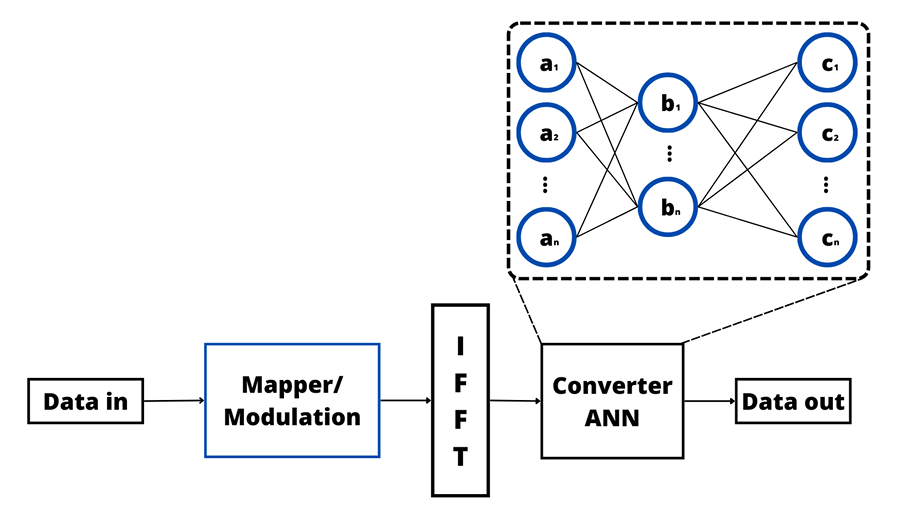
\includegraphics[width=0.70\linewidth]{Figures/09_ann_transmitter.png}
    \caption{An ANN-based OFDM transmitter for PAPR reduction.
             The neural network replaces or augments the classical SLM
             phase-sequence search.  The input is the frequency-domain
             OFDM symbol, and the output is the optimized signal.
             Reproduced from~\cite{da2024survey}.}
    \label{fig:ann_transmitter}
\end{figure}

\subsection{How Is an ANN Trained?}

Training is the process of finding the weights $\bm{W}$ and biases $\bm{b}$
that minimize a \textbf{loss function} $\mathcal{L}$.
The standard approach is \textbf{backpropagation} with
\textbf{gradient descent}~\cite{da2024survey}:

\begin{enumerate}
    \item \textbf{Forward pass:} feed an input through the network
          to produce an output.
    \item \textbf{Loss computation:} compare the output with the
          desired target using the loss function $\mathcal{L}$.
    \item \textbf{Backward pass (backpropagation):} compute the
          gradient $\partial\mathcal{L}/\partial w$ for every weight $w$
          using the chain rule.
    \item \textbf{Weight update:} adjust each weight in the direction
          that reduces the loss:
          \begin{equation}
              w \leftarrow w - \eta \frac{\partial\mathcal{L}}{\partial w},
              \label{eq:gradient_descent}
          \end{equation}
          where $\eta > 0$ is the \textbf{learning rate}.
    \item \textbf{Repeat} for many input samples (\textbf{epochs}) until
          the loss converges.
\end{enumerate}

\begin{misconception}
    \textbf{``Backpropagation is a separate algorithm from gradient descent.''} \\
    Backpropagation and gradient descent are two complementary parts of the
    same training process.  Backpropagation is the \emph{algorithm for
    computing gradients} (step~3 above); gradient descent is the
    \emph{algorithm for updating weights} using those gradients (step~4).
    Neither works without the other~\cite{da2024survey}.
\end{misconception}

\paragraph{Common Loss Functions for PAPR.}
The loss function is perhaps the most critical design choice for
PAPR-reduction networks, because it defines \emph{what} the network
learns to optimize.  The papers in this document use several variants:
\begin{itemize}
    \item \textbf{Mean Squared Error (MSE):}
          $\mathcal{L}_{\mathrm{MSE}} =
          \frac{1}{N}\sum_{n=0}^{N-1}|x(n) - \hat{x}(n)|^2$,
          where $\hat{x}$ is the network's output.
          Encourages signal fidelity (low BER)~\cite{kim2017novel,zou2021novel}.
    \item \textbf{PAPR loss:}
          $\mathcal{L}_{\mathrm{PAPR}} =
          \frac{\max_n|x(n)|^2}{\frac{1}{N}\sum_n|x(n)|^2}$
          or its log version.
          Directly penalizes high PAPR~\cite{kim2017novel,nguyen2022deep}.
    \item \textbf{Combined loss:}
          $\mathcal{L} = \alpha\,\mathcal{L}_{\mathrm{PAPR}} +
          (1-\alpha)\,\mathcal{L}_{\mathrm{MSE}}$,
          where $\alpha \in [0,1]$ balances PAPR reduction against
          signal distortion.  This joint formulation is a recurring
          theme across several papers~\cite{kim2017novel,zou2021novel}.
\end{itemize}

\paragraph{Common Optimizers.}
Instead of basic gradient descent, modern networks use adaptive optimizers:
\begin{itemize}
    \item \textbf{Adam}~\cite{kim2017novel,nguyen2022deep}:
          Combines momentum (exponential moving average of gradients)
          with RMSProp (adaptive per-parameter learning rates).
          The update rule is:
          \begin{align}
              m_t &= \beta_1 m_{t-1} + (1-\beta_1) g_t, \label{eq:adam_m}\\
              v_t &= \beta_2 v_{t-1} + (1-\beta_2) g_t^2, \label{eq:adam_v}\\
              w &\leftarrow w - \eta\,\frac{\hat{m}_t}{\sqrt{\hat{v}_t} + \epsilon}, \label{eq:adam_update}
          \end{align}
          where $g_t = \partial\mathcal{L}/\partial w$, and $\hat{m}_t$,
          $\hat{v}_t$ are bias-corrected estimates.
    \item \textbf{SGD with momentum}: used in some
          simpler architectures~\cite{hao2019extended}.
\end{itemize}


% ----------------------------------------------------------------------------
\section{Deep Neural Networks (DNNs)}
\label{sec:dnn}
% ----------------------------------------------------------------------------

A \textbf{Deep Neural Network} is simply an ANN with \emph{multiple}
hidden layers---typically three or more.  Depth is what gives DNNs
their expressive power: each layer learns increasingly abstract
representations of the input~\cite{da2024survey}.

\begin{figure}[htbp]
    \centering
    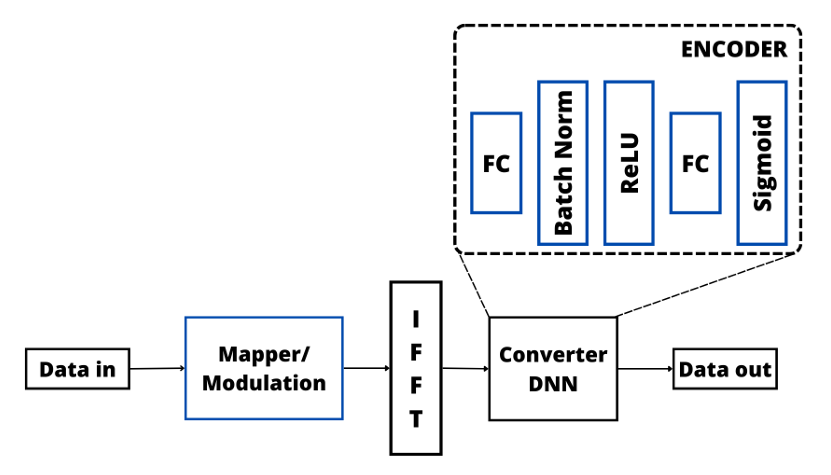
\includegraphics[width=0.70\linewidth]{Figures/10_dnn_transmitter.png}
    \caption{A DNN-based OFDM transmitter for PAPR reduction.
             Multiple hidden layers allow the network to learn complex
             nonlinear mappings from frequency-domain symbols to
             low-PAPR time-domain signals.
             Reproduced from~\cite{da2024survey}.}
    \label{fig:dnn_transmitter}
\end{figure}

\subsection{Training Challenges and Solutions}

Deep networks are harder to train than shallow ones.  Two key problems
and their solutions:

\paragraph{Vanishing/Exploding Gradients.}
During backpropagation, gradients are multiplied through each layer.
With many layers, these products can shrink exponentially
(vanishing gradients) or grow exponentially (exploding gradients),
stalling or destabilizing training~\cite{da2024survey}.

\textbf{Solutions used in our source papers:}
\begin{itemize}
    \item \textbf{ReLU activation:} gradients are either 0 or 1
          (no multiplicative shrinkage)~\cite{da2024survey,kim2017novel}.
    \item \textbf{Batch Normalization (BatchNorm):} normalizes the inputs
          to each layer to have zero mean and unit variance.
          For a mini-batch of activations $\{z_i\}_{i=1}^{m}$:
          \begin{equation}
              \hat{z}_i = \frac{z_i - \mu_B}{\sqrt{\sigma_B^2 + \epsilon}},
              \qquad
              y_i = \gamma\,\hat{z}_i + \beta,
              \label{eq:batchnorm}
          \end{equation}
          where $\mu_B$ and $\sigma_B^2$ are the mini-batch mean and variance,
          and $\gamma$, $\beta$ are learnable scale and shift parameters.
          BatchNorm stabilizes training and allows higher learning
          rates~\cite{kim2017novel}.
    \item \textbf{Proper weight initialization:} Xavier or He initialization
          sets initial weights to have variance scaled by the layer
          size, keeping activation magnitudes stable through the
          network~\cite{da2024survey}.
\end{itemize}

\paragraph{Overfitting.}
A network with millions of parameters can memorize the training data
rather than learning generalizable patterns.

\textbf{Solutions used in our source papers:}
\begin{itemize}
    \item \textbf{Dropout:} during training, randomly set a fraction $p$
          of neuron outputs to zero at each forward pass.
          This forces the network to learn redundant representations
          that are robust to missing features~\cite{kim2017novel}.
    \item \textbf{Early stopping:} monitor performance on a validation set
          and stop training when it starts degrading.
    \item \textbf{Large training datasets:} generate a large number of
          random OFDM symbols for training
          (e.g., $10^5$--$10^6$ symbols)~\cite{kim2017novel,zou2021novel}.
\end{itemize}

\begin{keyinsight}
    A key advantage of applying DNNs to PAPR reduction is that
    \emph{training data is free}: we can generate as many random
    OFDM symbols as we want by drawing constellation points from
    the modulation alphabet.  There is no need for expensive data
    collection because the signal model is known analytically~\cite{da2024survey}.
\end{keyinsight}


% ----------------------------------------------------------------------------
\section{Autoencoders (AEs)}
\label{sec:autoencoders}
% ----------------------------------------------------------------------------

An \textbf{autoencoder} is a neural network trained to reproduce its input
at the output while forcing the data through a \textbf{bottleneck} in the
middle.  The network has two halves~\cite{da2024survey,kim2017novel}:

\begin{itemize}
    \item \textbf{Encoder} $g_\theta(\cdot)$:
          compresses the input $\bm{x}$ into a lower-dimensional
          \textbf{latent representation} $\bm{h}$:
          \begin{equation}
              \bm{h} = g_\theta(\bm{x}),
              \qquad \bm{h} \in \mathbb{R}^{d_h},\; d_h < d_x.
              \label{eq:encoder}
          \end{equation}
    \item \textbf{Decoder} $f_\phi(\cdot)$:
          reconstructs the original input from the latent representation:
          \begin{equation}
              \hat{\bm{x}} = f_\phi(\bm{h}) = f_\phi\bigl(g_\theta(\bm{x})\bigr).
              \label{eq:decoder}
          \end{equation}
\end{itemize}

The autoencoder is trained end-to-end to minimize the reconstruction error:
\begin{equation}
    \mathcal{L}_{\mathrm{AE}} =
    \frac{1}{N}\sum_{i=1}^{N}\bigl\|\bm{x}_i - \hat{\bm{x}}_i\bigr\|^2.
    \label{eq:ae_loss}
\end{equation}

\begin{workingexample}[Analogy: Summarize and Reconstruct]
    Imagine you must describe a 100-word paragraph to a friend using
    only 10 words (the bottleneck), and your friend must then reconstruct
    the full paragraph from your 10-word summary.  An autoencoder learns
    to create the \emph{most informative possible summary} (encoder) and
    the \emph{best possible reconstruction strategy} (decoder).
\end{workingexample}

\subsection{Why Autoencoders for PAPR Reduction?}

The autoencoder framework maps naturally onto the OFDM communication
chain~\cite{kim2017novel,alnaseri2025deep}:

\begin{itemize}
    \item The \textbf{encoder} plays the role of the transmitter:
          it maps data symbols to a transmitted signal representation.
    \item The \textbf{channel} (noise, fading) sits between encoder
          and decoder.
    \item The \textbf{decoder} plays the role of the receiver:
          it recovers the original data from the received signal.
\end{itemize}

By incorporating a PAPR penalty into the loss function, the encoder
is forced to learn representations that are simultaneously
\emph{low-PAPR} and \emph{recoverable by the decoder}.
This is exactly what SLM tries to achieve with hand-crafted phase
sequences, but the autoencoder learns the optimal ``phase sequences''
automatically~\cite{kim2017novel,hao2019extended}.

\begin{keyinsight}
    The autoencoder framework is the \emph{most common} ML architecture for
    PAPR reduction in our source papers.
    Three of the seven papers---Kim~2017~\cite{kim2017novel},
    Hao~2019~\cite{hao2019extended}, and
    Alnaseri~2025~\cite{alnaseri2025deep}---build on this paradigm,
    each extending it in a different direction.
\end{keyinsight}


% ----------------------------------------------------------------------------
\section{Deep Unfolding Networks}
\label{sec:deep_unfolding}
% ----------------------------------------------------------------------------

\subsection{The Core Idea: Unrolling an Iterative Algorithm}

Many classical signal processing algorithms are \textbf{iterative}:
they repeat a fixed update rule until convergence.
For example, the iterative clipping-and-filtering (ICF) algorithm for
PAPR reduction repeats ``clip $\to$ filter $\to$ check convergence''
for a fixed number of iterations~\cite{nguyen2022deep}.

\textbf{Deep unfolding} takes such an iterative algorithm, ``unrolls'' it
for a fixed number of $L$ iterations, and replaces some of the hand-tuned
parameters (e.g., step sizes, thresholds) with \textbf{learnable parameters}
optimized via backpropagation~\cite{nguyen2022deep}:

\begin{equation}
    \text{Classical: } \bm{x}^{(\ell+1)} = \mathcal{T}\!\bigl(\bm{x}^{(\ell)};\,\lambda\bigr),
    \qquad
    \text{Unfolded: } \bm{x}^{(\ell+1)} = \mathcal{T}\!\bigl(\bm{x}^{(\ell)};\,\theta_\ell\bigr),
    \label{eq:unfolding}
\end{equation}
where $\lambda$ is a fixed hand-tuned parameter and $\theta_\ell$ is a
\emph{layer-specific} learnable parameter.

\begin{workingexample}[Analogy: Tuning a Recipe]
    Classical iterative algorithms are like following a recipe with
    fixed cooking times and temperatures.  Deep unfolding is like
    following the same recipe structure, but allowing each step's
    time and temperature to be independently optimized based on
    tasting results.  You keep the \emph{structure} of the recipe
    (the algorithm), but \emph{learn} the best parameters for each step.
\end{workingexample}

\subsection{Advantages Over Purely Data-Driven Networks}

Deep unfolding offers a compelling middle ground between purely
classical and purely data-driven approaches~\cite{nguyen2022deep}:

\begin{enumerate}
    \item \textbf{Interpretability:} each layer corresponds to one iteration
          of a known algorithm, so the network's behavior is understandable.
    \item \textbf{Parameter efficiency:} instead of millions of free parameters
          (as in a generic DNN), the unfolded network has only a few
          learnable parameters per layer (e.g., step sizes and thresholds),
          dramatically reducing the number of trainable weights.
    \item \textbf{Convergence speed:} because the structure encodes domain
          knowledge, the network requires far less training data and
          converges faster than a black-box DNN~\cite{nguyen2022deep}.
    \item \textbf{Guaranteed structure:} physical constraints
          (e.g., power constraints, subcarrier masks) can be
          hard-coded into the unfolded layers.
\end{enumerate}


% ----------------------------------------------------------------------------
\section{Genetic Algorithms (GAs)}
\label{sec:genetic_algorithms}
% ----------------------------------------------------------------------------

\subsection{Overview: Optimization Inspired by Natural Evolution}

A \textbf{Genetic Algorithm (GA)} is a meta-heuristic optimization method
that mimics the process of natural selection~\cite{ali2016new}.
Unlike neural networks, GAs do not learn from labeled data---instead,
they evolve a \textbf{population} of candidate solutions toward
an optimum through three biological operators:

\begin{enumerate}
    \item \textbf{Selection:} evaluate each candidate using a
          \textbf{fitness function} and preferentially select the
          fittest individuals for reproduction.
    \item \textbf{Crossover (recombination):} combine pairs of selected
          candidates to produce offspring that inherit traits from
          both parents.
    \item \textbf{Mutation:} randomly alter some genes (parameters)
          in offspring to introduce diversity and prevent premature
          convergence.
\end{enumerate}

\begin{workingexample}[Analogy: Breeding Racing Pigeons]
    A GA for SLM is like breeding racing pigeons.  Each pigeon (candidate)
    is a phase sequence, and its speed (fitness) is the resulting PAPR.
    You keep the fastest pigeons (selection), breed them together
    (crossover to combine good traits), and occasionally introduce
    random variation (mutation) to explore new possibilities.
    After many generations, the population converges toward very fast
    pigeons---or in our case, very low-PAPR phase sequences.
\end{workingexample}

\subsection{GA for SLM: Encoding and Fitness}

In the context of SLM~\cite{ali2016new}:
\begin{itemize}
    \item \textbf{Chromosome:} a phase sequence
          $\bm{\psi} = [\psi_0, \psi_1, \dots, \psi_{N-1}]^T$.
    \item \textbf{Gene:} a single phase factor $\psi_k$.
    \item \textbf{Population:} a set of $P$ phase sequences (chromosomes).
    \item \textbf{Fitness function:} the negative PAPR (since we want to
          \emph{minimize} PAPR, and GAs conventionally \emph{maximize}
          fitness):
          \begin{equation}
              \mathcal{F}(\bm{\psi}) = -\mathrm{PAPR}\bigl(\mathrm{IFFT}\{\bm{X} \odot \bm{\psi}\}\bigr).
              \label{eq:ga_fitness}
          \end{equation}
\end{itemize}

The GA iterates through selection, crossover, and mutation for a fixed
number of \textbf{generations} (iterations) $G$.  After $G$ generations,
the fittest individual (the phase sequence producing the lowest PAPR)
is used for transmission~\cite{ali2016new}.

\begin{keyinsight}
    The GA approach does \emph{not} require training data or a neural
    network.  It is an optimization algorithm that runs \emph{at
    transmission time} for each OFDM symbol.  This is fundamentally
    different from the DNN-based approaches, which train offline and
    perform fast inference online.  The trade-off is that the GA's
    per-symbol computational cost can be high if many generations
    are needed~\cite{ali2016new}.
\end{keyinsight}


% ----------------------------------------------------------------------------
\section{Summary: Which ML Tool for Which SLM Problem?}
\label{sec:ml_summary}
% ----------------------------------------------------------------------------

Table~\ref{tab:ml_tools_mapping} maps each ML technique to the SLM
limitation(s) it addresses and the specific papers that employ it.

\begin{table}[htbp]
    \centering
    \caption{Mapping of ML techniques to SLM limitations and source papers.}
    \label{tab:ml_tools_mapping}
    \begin{tabularx}{\textwidth}{@{} >{\raggedright\arraybackslash}p{2.5cm} >{\raggedright\arraybackslash}X >{\raggedright\arraybackslash}p{2cm} >{\raggedright\arraybackslash}p{2.5cm} @{}}
        \toprule
        \textbf{ML Technique} & \textbf{SLM Limitation Addressed} & \textbf{Training} & \textbf{Papers} \\
        \midrule
        ANN / DNN &
            Complexity reduction; replaces $U$ IFFTs with single forward pass &
            Offline &
            \cite{da2024survey,zou2021novel} \\[6pt]
        Autoencoder &
            Complexity + SI elimination; learns joint Tx/Rx &
            Offline &
            \cite{kim2017novel,hao2019extended,alnaseri2025deep} \\[6pt]
        Deep Unfolding &
            Complexity + intelligent search; unrolls iterative PAPR algorithm &
            Offline &
            \cite{nguyen2022deep} \\[6pt]
        Genetic Algorithm &
            Intelligent search; evolves optimal phase sequences &
            None (online) &
            \cite{ali2016new} \\
        \bottomrule
    \end{tabularx}
\end{table}

With this ML toolkit in hand, we are ready to study each approach in
detail.  The next chapter examines the \emph{first} deep-learning-based
PAPR reduction method: Kim et al.'s PRNet autoencoder~\cite{kim2017novel}.
